\section{alexander}

\comm{Davenma y Venema}

\comm{En la claim 2.1.5 usar la descomposición de heegaard de $\R^3$ como dos toros}

\comm{Al final de los ejemplos hablar de que tomar suspensión me da ejemplos de dim superior. Esto está en DV después de Alexander.}

En esta sección vamos a dar un ejemplo de una bola encajada en $\R^3$ tal que el encaje no se extiende a un homeomorfismo de todo $\R^3$. 

Podemos construir la imagen como una intersección numerable de cerrados encajados $\{X_n\}$. Para el resto de la construcción, va a ser conveniente definir los siguientes conjuntos auxiliares: 

Sea $T$ un toro sólido estándar en $\R^3$ dado por un encaje $\varphi :\s^1\times \D^2\rightarrow \R^3$ y sea $[t_1,t_2]\subset \s^1$ un intervalo cerrado. Llamamos cilindro al conjunto $C:=\varphi([t_1,t_2]\times \D^2)$, y decimos que las tapas del cilindro son los dos discos $\tau_1 := \varphi(\{t_1\}\times\D^2)$, $\tau_2 := \varphi(\{t_2\}\times\D^2)$.

Dado un cilindro $C$, consideramos dos toros sólidos disjuntos y enlazados $T_1$, $T_2$ contenidos en $C$ tales que $T_1\cap \partial C=\tau_1$, $T_2\cap \partial C=\tau_2$ como en la imagen $\ref{alex1}$. 

\comm{los toros tienen número de enlace 1, ver si defino número de enlace o cómo digo eso. todos los enlaces que voy a usar siempre van a ser simples, o sea van a tener número de enlace 1. seguro esta construcción se puede hacer con número de enlace arbitrario y tiene pinta que quedan no equivalentes}

\begin{figure}[h!]
    \centering
    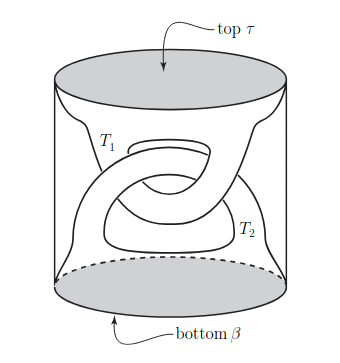
\includegraphics[width=0.5\linewidth]{img mono/alexander/1.png}
    \caption{Un cilindro conteniendo $T_1$ y $T_2$}
    \label{alex1}
\end{figure}

Ahora si, vamos a definir nuestra sucesión de cerrados encajados: 

Empezamos por $X_0$ un toro sólido estándar en $\R^3$. Identificamos en su interior un cilindro $C_0$ con dos toros enlazados $T_1$ y $T_2$, definimos $X_1:=(X_0-C)\cup T_1\cup T_2$.

Para definir $X_2$, vamos a modificar sólamente los toros $T_1$ y $T_2$, y lo haremos de la misma forma en la que modificamos el toro $X_0$ en el paso anterior. Lo que hacemos es considerar dos cilindros $C_1\subset T_1$ y $C_2\subset T_2$, esta vez teniendo en cuenta que $\tau_1\cap C_1=\varnothing$ y $\tau_2\cap C_2=\varnothing$, es decir, que no corten a las tapas del cilindro anterior. Definimos $X_2$ como $X_1-(C_1\cup C_2)$ unido con los $4$ subtoros contenidos en $C_1$ y $C_2$.

Seguimos iterando este proceso, 
            
Repito este proceso con $T_1$ y $T_2$, y al resultado lo llamo $X_3$. Observamos que $X_n$ van quedando encajadas. Seguimos haciendo esto procurando hacer que
tachado: los diámetros internos de los $T_i$ tiendan a 0 los diámetros de las pillboxes tiendan a $0$ y llamamos $B=\bigcap\limits_{n=1}^\infty X_n$, esta es la bola de Alexander. 

Llamamos $S=\partial B$ la esfera de Alexander. 

Veamos que $\pi_1(B^c)\neq\{1\}$: Tomamos $J$ una curva cerrada que es no trivial en el complemento de $X_1$ (toro). Supongamos $J$ es trivial en $B^c$ y consideramos su homotopía $H$ a un punto. 
            
$Im(H)$ es un compacto tal que $Im(H)\subset B^c=\left(\bigcap\limits_{n=1}^\infty X_n\right)^c=\bigcup\limits_{n=1}^\infty X_n^c$. Observamos que $\{X_n^c\}$ es una familia de abiertos encajados, y por lo tanto $Im(H)$ está contenida en una cantidad finita de ellos. 

Esto implica que existe un $N\in\N$ tal que $Im(H)\subset X_N^c$, es decir, $J$ es contractible en $X_N^c$. Por inducción podemos ver que esto es absurdo. 

Ahora veamos que $B$ es una 3-célula: Pensemos $B$ como unión de cosas en vez de intersección. 

En la etapa $n$ de la construcción tenemos $2^{n-1}$ pillboxes, que cada una contiene 2 toros sólidos. Tenemos entonces $2^n$ toros sólidos en la etapa $n$, que son cada uno unión de una pillbox y una 3-célula complementaria. 

Definimos $D_n$ a la unión de las $2^{n-1}$ 3-células complementarias a las $2^{n-1}$ pillboxes en la etapa $n$ de la construcción. 

De esta manera podemos definir $B$ como $\overline{\bigcup\limits_{n=1}^\infty C_n}$, siendo $C_1=D_1$ y $C_n=C_{n-1}\cup D_n$ 
            
\duda{convencerme de por qué preciso clausurar--> $B$ es intersección arbitraria de cerrados entonces es cerrado, los $C_n$ son abiertos entonces su unión va a ser abierta. Como $B$ no es $\varnothing$ ni $\R^3$ no puede ser un clopen, entonces no son iguales. Falta convencerme pq clausurar funciona.} 

Llamemos $P_n^i$ a la i-ésima pillbox del n-ésimo paso de la construcción. Es decir, $P_n^i\subset X_n \fall i\in\{1,\dots,2^{n-1}\}$ y $X_n=X_{n+1}\cup\bigcup\limits_{i=1}^{2^{n-1}}P_n^i$. 
            
Sea $x\in B-\bigcup\limits_{n=1}^\infty C_n \Rightarrow x\in \bigcap\limits_{n=1}^\infty X_n-\bigcup\limits_{n=1}^\infty C_n$ 

$x\not\in\bigcup\limits_{n=1}^\infty C_n \Rightarrow x\not\in C_n\fall n\in\N$ 

$x\in B-C_n\Rightarrow \exst i\in\{1,\dots,2^{n-1}\}$ tal que $x\in P_n^i$ 

Con esto concluimos que $x\in B-\bigcup\limits_{n=1}^\infty C_n \Leftrightarrow x\in\bigcap\limits_{n=1}^\infty P_n^{k_n}$ para alguna sucesión de naturales $\{k_n\}$. \comm{recordar que $diam(P_n)\xrightarrow{n} 0$, son compactas y encajadas}

Como $diam(P_n)\xrightarrow{n} 0$, esto además implica que $x\in\overline{\bigcup\limits_{n=1}^\infty C_n}$, y por lo tanto tenemos la igualdad de conjuntos. 

Además, fun fact, observar que dada una pillbox $P_n^i$ se cumple que $\#\big\{j\in\{1,\dots, 2^n\}:P_{n+1}^j\cap P_n^i\neq\varnothing\big\}=2$, por lo tanto, los $x\in B-\bigcup\limits_{n=1}^\infty C_n$ están en biyección con $2^{\N}$, es decir, son un Cantor. 

Viendo $B$ de esta manera, probemos que efectivamente es una bola: 

Para cada $C_n$ en la construcción, podemos definir un homeo $h_n:C_n\to C_{n+1}$ soportado en un entorno $U_n$ de $C_n\cap D_{n+1}$. 

Definimos entonces una familia de funciones $\{f_n:C_1\to C_{n+1}\}_{n\in\N}$ tales que $f_n=h_n\circ h_{n-1}\circ\dots\circ h_1$. Observar que cada $f_n$ difiere de $f_{n+1}$ sólamente en $U_n$.

Como $diam(P_n)\xrightarrow n 0$, podemos ir tomando los $U_n$ con $diam(U_n)\xrightarrow n 0$, por lo tanto $\{f_n\}$ converge uniformemente a $f:C_1\to B$, que resulta continua. \comm{acomodar esto pq en realidad los $U_n$ son disconexos entonces el diametro no tiende a 0}

Queremos verificar ahora que $f$ es biyectiva, y con eso obtener que es un homeomorfismo. 

Por lo visto anteriormente, sabemos que $K=f^{-1}(B-\bigcup\limits_{n=1}^{\infty}C_n)$ es un conjunto de Cantor. 

Dado $x\in C_1- K$, $\exst N\in\N$ tal que $f_{N-1}(x)\in C_{N}-U_N$ (en este caso pensamos $f_0$ como la identidad), y por lo tanto $f(x)=f|_{N-1}(x)$. 
            
Con esto tenemos que $f$ es biyectiva en $C_1- K$. 

Por lo observado anteriormente, dados $x_0, x_1\in K$, en algún momento van a estar en distintas componentes conexas de los entornos $U_n$, y por lo tanto van a diferir sus imágenes por alguna de las $f_n$. Con esto tenemos la inyectividad de $f$ en $K$. 

Para la sobreyectividad, tomamos un punto $x\in B-\bigcup\limits_{n=1}^{\infty}C_n$ y su correspondiente elemento de $2^\N$, y observamos que se corresponde a un único punto \comm{terminar de escribir}
